\chapter{Network Layer}

\section{Routing}
\textbf{Routing:} Routing is the process of selecting a path for data to travel from a source to a destination across interconnected networks. It ensures data packets are delivered efficiently through the best possible route.

\textbf{Router:} A router is a networking device that connects multiple networks together and forwards data packets between them based on their destination IP address. It makes routing decisions using routing tables and protocols.

\begin{figure}[H]
   \centering
   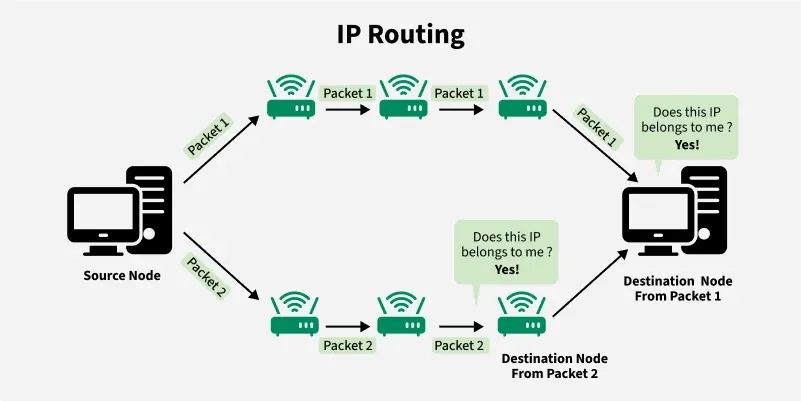
\includegraphics[width=0.6\textwidth]{figures/Routing.png}
\end{figure}

\section{Difference between Static and Dynamic Routing}
\begin{tabularx}{\textwidth}{|X|X|}
   \hline
   \thc{Static Routing} & \thc{Dynamic Routing} \\\hline
   Routes are user-defined. & Automatically adjusted based on network conditions. \\\hline
   Does not use complex routing algorithms. & Uses complex routing algorithms to determine the best path. \\\hline
   Provides high security. & Less secure. \\\hline
   Does not require additional resources. & Require additional resources. \\\hline
   Failure of the link disrupts the rerouting. & Failure of the link doesn't disrupts the rerouting. \\\hline
   Requires less bandwidth. & Requires more bandwidth. \\\hline
\end{tabularx}


\section{Network Address Translation (NAT)}
\begin{wrapfigure}{r}{0.5\textwidth}
   \centering
   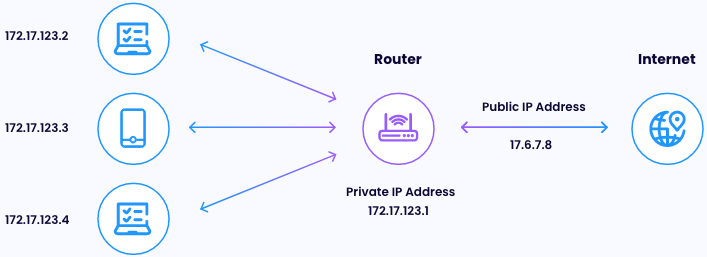
\includegraphics[width=\linewidth]{figures/NAT.png}
\end{wrapfigure}
Network Address Translation (NAT) is a process in which one or more local IP addresses are translated into one or more Global IP addresses and vice versa to provide Internet access to the local hosts. It also does the translation of port numbers, i.e., masks the port number of the host with another port number in the packet that will be routed to the destination. It then makes the corresponding entries of IP address and port number in the NAT table. NAT generally operates on a router or firewall.


\section{Main Routing Protocols}

% \subsection{RIP (Routing Information Protocol)}
% RIP is a distance-vector routing protocol that uses hop count as its metric (max 15 hops). Based on the Bellman-Ford algorithm, it periodically broadcasts the updates of the network that the full routing table. RIP v1 is classful; RIP v2 is classless and supports subnetting and authentication. It suits small networks but has slow convergence and limited scalability.

% \textbf{OSPF (Open Shortest Path First)}: OSPF is a link-state protocol that finds the shortest path using the Dijkstra algorithm.

\begin{tabularx}{\textwidth}{|X|X|}\hline
   \thc{RIP (Routing Information Protocol)} & \thc{OSPF (Open Shortest Path First)} \\\hline

   A distance-vector routing protocol that uses hop count (max 15 hops) to determine the best path between routers. &
   A link-state routing protocol that uses a map of the network and calculates the shortest path between routers. \\\hline

   RIP uses Bellman-Ford algorithm & OSPF uses Dijkstra algorithm. \\\hline

   % Broadcasts the full routing table to its neighbors every 30s. & OSPF sends updates only when there is a change in the network topology, reducing bandwidth usage. \\\hline

   Broadcasts entire routing table to all neighbors every 30s. This is also known as Routing on rumors. & Multicasts only changes using LSAs only when there is a change in the network topology.
   \\\hline


   RIP v1: Classful, RIP v2: Classless & Classless (supports VLSM and CIDR)   \\\hline

   Suitable for small networks. & Suitable for larger networks. \\\hline
   
   Slow convergence. & Faster convergence. \\\hline

   Uses UDP (Port 520) &
   Runs directly over IP (Protocol number 89)
   \\\hline
\end{tabularx}

\vspace{2em}
\textbf{EIGRP (Enhanced Interior Gateway Routing Protocol)}: It is a hybrid protocol that combines features of
distance-vector and link-state.

\textbf{BGP (Border Gateway Protocol)}: It is a path-vector protocol that is used for routing between different
autonomous systems on the internet.

\textbf{Distance Vector Routing}: All the nodes that are a part of the network advertise their routing table to their
adjacent nodes (nodes that are directly connected) at regular intervals. Algorithm used: Bellman Ford
Algorithm to find the shortest path.

\section{Difference Between IPv4 and IPv6}
\begin{tabularx}{\textwidth}{|l|X|X|}\hline
   \thc{Property} & \thc{IPv4} & \thc{IPv6} \\\hline
   Address Length & 32 bits (decimal representation) & 128 bits (hexadecimal representation) \\\hline
   Address configuration & Manual and DHCP & Auto and renumbering \\\hline
   Connection integrity & unachievable end to end connection integrity & achievable end to end connection integrity\\\hline
   Encryption \& Auth & not provided by default & provided by default \\\hline
   Security & dependent on application & built-in security features (IPSec) \\\hline
   Header size & 20-60 bytes (variable) & 40 bytes (fixed) \\\hline
   Subnetting & Supports VLSM & Doesn't supports VLSM \\\hline
   Example & 66.94.29.13 & 2001:0000:3238:DFE1:0063:0000:0000:A0F8 \\\hline
\end{tabularx}